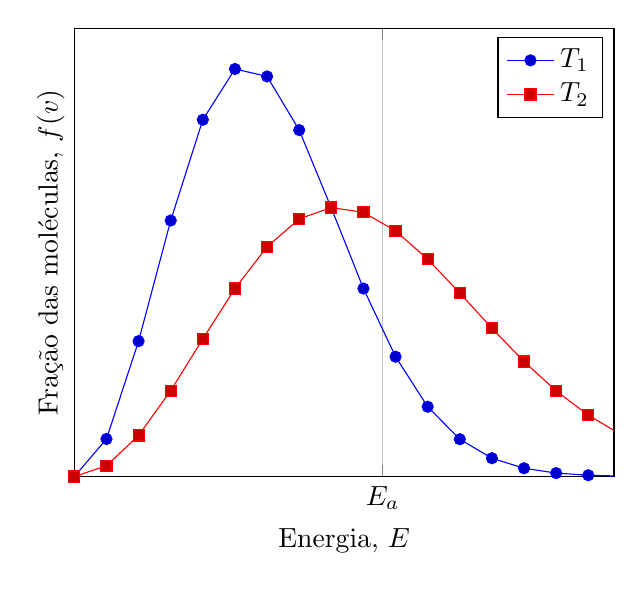
\begin{tikzpicture}
    \def\R{1000*8.314}% boltzmann constant
    \begin{axis}
        [
            domain = 0:5000,
            xlabel = {Energia, $E$},
            ylabel = {Fração das moléculas, $f(v)$},
            xtick={2000}, 
            xticklabels = {$E_\text{a}$},
            grid = major,
            ytick=\empty,
            xmin=0, ymin=0,
            xmax=3500,
        ]
    \pgfplotsinvokeforeach{300,700}
    {
        \addplot
        {
            sqrt(2/pi)*(4/(\R*#1))^(3/2)*x^2*exp(-4/(\R*#1)*x^2/2)
        };
    }
    \legend{$T_1$, $T_2$}
\end{axis}
\end{tikzpicture}